
%--------------------------------------------------------
%--------------------------------------------------------
%--------------------------------------------------------
%--------------------------------------------------------
\section{Úvod}

Pro popis trojrozměrné scény z~každého možného úhlu lze definovat plenoptickou funkci $\mathrm{P}(x,y,z,\phi,\psi)$, kde $(x,y,z)$ je pozice a~$(\phi,\psi)$ je pozorovací úhel.
Hodnota $\mathrm{P}$ určuje intenzitu světelného paprsku.
Definici lze dále rozšířit o~$t$ (čas) pro popsání dynamické scény.
Tato práce pracuje s~fotografiemi pořízenými polem fotoaparátů nebo jedním senzorem, který je předcházen polem mikročoček.
Oba případy lze reprezentovat jako pohledy na scénu uspořádané v~pravidelné mřížce v~rovině.
Tato reprezentace je často nazývána 4D světelné pole a~lze jej popsat funkcí $\mathrm{L}(u,v,s,t)$, kde $(u,v)$ jsou pro\-s\-torové souřadnice (souřadnice pohledu) a~$(s,t)$ jsou původní úhlové souřadnice (souřadnice pixelu).

Světelné pole implicitně zachovává informace o~pro\-s\-torových i~materiálových vlastnostech ve scéně.
Jelikož jde světelné pole zaznamenat i~zobrazit jak v~reálném, tak v~digitálním světě, lze jej považovat za pro\-stře\-dek komunikace vizuálních dat mezi těmito světy.
Důležitým aspektem světelných polí, který je potřeba řešit, je jejich paměťová náročnost.

Na světelné pole se lze dívat jako na pole běžných, avšak silně korelovaných obrazových snímků.
Je zřejmé, že tato korelace nemůže v~případě kom\-pre\-se zůstat bez povšimnutí.
Ukázalo se, že společně s~korelací v~obrazové rovině lze korelaci mezi pohledy dobře využít při kom\-pre\-si na bázi 4D bloků~\cite{Dlabaja2018}.
Tato bloková komprese byla srovnána s~ostatními kompresními metodami~\cite{Barina2019}, kde byla ve většině případů překonána.
Této me\-to\-dě uniká ně\-ko\-lik aspektů, které mají vliv na úroveň kom\-pre\-se.

Jedna z~věcí, kterou lze pro kom\-pre\-si využít, je korelace mezi sousedními bloky.
Stejně jako u~2D obrazových dat, i~u~světelných polí platí, že krajní vzorky sousedních bloků jsou s~velkou pravděpodobností podobné obsahu aktuálně komprimovaného bloku.
Obsah bloku lze proto zaznamenat jako me\-to\-du pre\-dikce právě komprimovaného bloku s~využitím již zakódovaných vzorků a~chyby, které se tato pre\-dikce dopustila (rezidua, rozdílu).
Při správné volbě směr\-ového vektoru je zakódovaná chyba pre\-dikce společně s~me\-to\-dou menší, než data kódovaná bez pre\-dikce, a~dojde tak ke kom\-pre\-si dat.
Návrhu takového pre\-dikčního schématu pro 4D světelná pole se věnuje kapitola~\ref{pred}.
Navržená me\-to\-da je zaměřená na univerzálnost použití, její přímou implementaci tak lze například použít v~kom\-bi\-na\-ci s~hyperbloky libovolných roz\-měrů.

Dalším aspektem je tvar a~velikost hyperbloků.
U~2D obrázků lze bezpečně předpokládat, že data budou mít stejnou povahu ve vertikálním i~horizontálním směru.
Taková data lze komprimovat po čtvercových blocích, jiné roz\-měry by ve většině případů nepřinesly zlepšení.
Pro 4D světelná pole je však situace jiná.
Data mají podobnou povahu navzájem v~úhlových souřadnicích a~navzájem v~pro\-s\-torových souřadnicích, ale ne mezi úhlovými a~pro\-s\-torovými souřadnicemi.
Dává proto smysl používat bloky, které mají v~pro\-s\-torových a~úhlových souřadnicích rozdílnou velikost.
Implementaci kom\-pre\-se s~hyperbloky obecných roz\-měrů se věnuje kapitola~\ref{hyperbloky}.

Třetím zkoumaným vlivem je disparita mezi po\-hledy.
Experimenty ukázaly, že pro blokovou me\-to\-du je maximální dosažitelná úroveň kom\-pre\-se korelována s~disparitou mezi po\-hledy.
Platí, že světelná pole s~menší disparitou lze komprimovat lépe než světelná pole s~větší disparitou.
Bylo proto otázkou, jestli nejde před samotnou kom\-pre\-sí minimalizovat disparitu v~obrázku tak, aby došlo k~lepší kom\-pre\-si beze ztráty dat.
Tato hypotéza se ukázala jako platná.
Metoda, která disparitu minimalizuje, je popsána v~kapitole~\ref{disp}.

Kodek s~popsanými modifikacemi překonává state-of-the-art metody pro videokompresi pro obrázky s~nižší disparitou (Lytro, Stanford).
Pro obrázky s~vyšší disparitou (Stanford, SAUCE) metoda překonává state-of-the-art metody při kompresi s~kvalitou vyšší než ~43 dB PSNR.

\section{Intra pre\-dikce pomocí směr\-ových vektorů}\label{pred}

\begin{figure}[htbp]\centering
  \centering
  \subcaptionbox{\label{dost-a}}{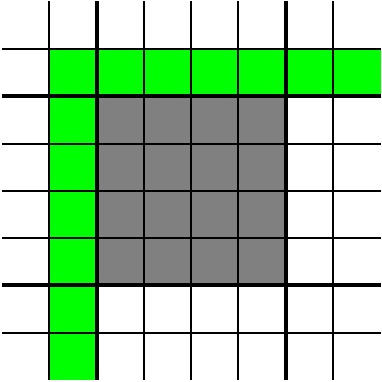
\includegraphics[width=8cm/2]{dost-predp.pdf}}
  \hfill
  \subcaptionbox{\label{dost-b}}{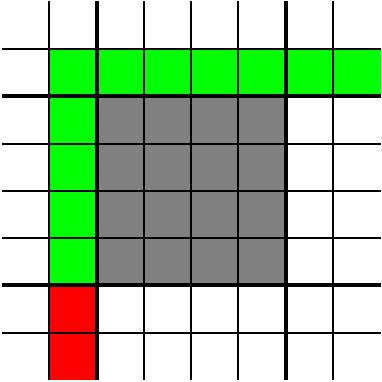
\includegraphics[width=8cm/2]{dost-real.pdf}}
  \vspace*{1em}
  \caption{Obrázek~\ref{dost-a} zeleně demonstruje vzorky, jejichž existenci pre\-diktor předpokládá.
  Obrázek~\ref{dost-b} červeně značí vzorky, které nejsou dostupné na straně dekodéru při scanline průchodu.
  Přístup k~nedostupnému vzorku řeší uživatel, optimální strategie je vracet nejbližší dostupný vzorek.}
  \label{fig:dost}
\end{figure}

\begin{figure}[htbp]\centering
  \centering
  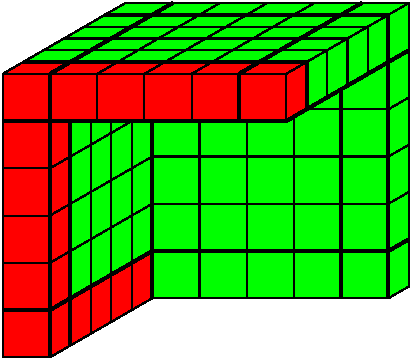
\includegraphics[width=8cm/2]{3d.pdf}
  \caption{Ve třech roz\-měrech se scanline průchod komplikuje. Na první po\-hled není zřejmé, které vzorky jsou dostupné na straně dekodéru.}
  \label{fig:dost-3D}
\end{figure}

\begin{figure*}[htbp]\centering
  \centering
  \subcaptionbox{\label{kv-a}}{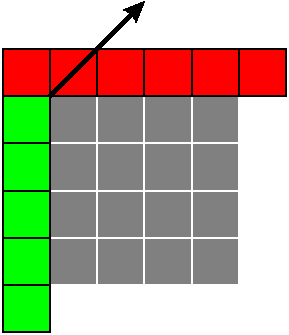
\includegraphics[width=6cm/2]{kv1.pdf}}
  \hfill
  \subcaptionbox{\label{kv-b}}{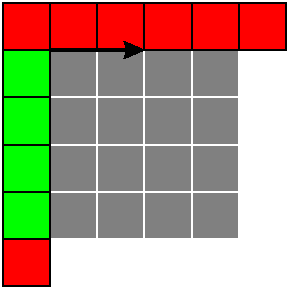
\includegraphics[width=6cm/2]{kv1-2.pdf}}
  \hfill
  \subcaptionbox{\label{kv-c}}{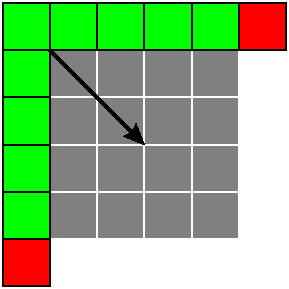
\includegraphics[width=6cm/2]{kv2.pdf}}
  \hfill
  \subcaptionbox{\label{kv-d}}{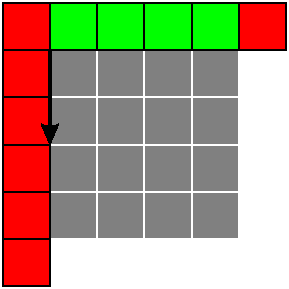
\includegraphics[width=6cm/2]{kv2-3.pdf}}
  \hfill
  \subcaptionbox{\label{kv-e}}{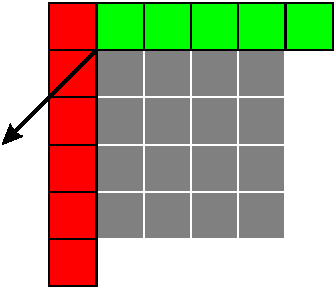
\includegraphics[height=6cm/2]{kv3.pdf}}
  \vspace*{1em}
  \caption{Zeleně jsou označeny vzorky, které bude pre\-diktor pro daný směr číst. Prediktor nikdy nečte červeně označené vzorky. Uživatel se na toto chování může spolehnout a~nemusí provádět dodatečné kontroly.}
  \label{fig:kv}
\end{figure*}

\begin{figure}[htbp]\centering
  \centering
  \subcaptionbox{\label{okraj-a}}{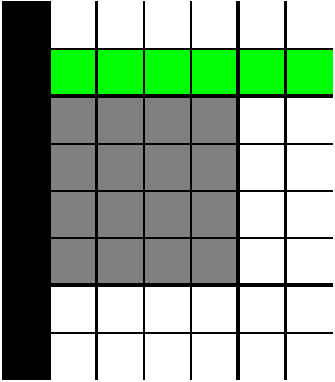
\includegraphics[width=7cm/2]{okraj-levy.pdf}}
  \hfill
  \subcaptionbox{\label{okraj-b}}{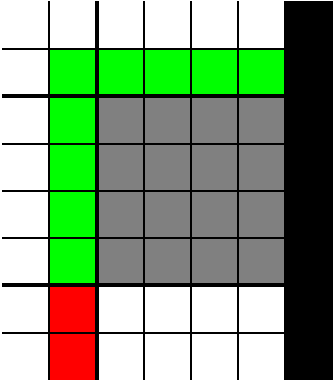
\includegraphics[width=7cm/2]{okraj-pravy.pdf}}
  \vspace*{1em}
  \caption{Obrázky~\ref{okraj-a} a~\ref{okraj-b} demonstrují případy, kdy je pre\-dikovaný blok okrajem obrázku. Začerněné vzorky nejsou dostupné ani na straně kodéru.
  Přístup k~nedostupnému vzorku řeší uživatel, optimální strategie je vracet nejbližší dostupný vzorek.
  Vertikální okraje jsou řešeny obdobně.}
  \label{fig:okraj}
\end{figure}

\begin{figure*}[htbp]\centering
  \centering
  \subcaptionbox{\label{okt-a}}{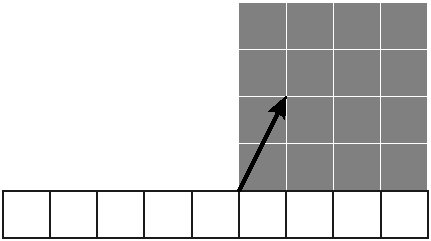
\includegraphics[width=9cm/2]{okt1.pdf}}
  \hfill
  \subcaptionbox{\label{okt-b}}{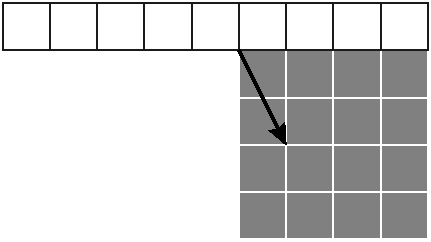
\includegraphics[width=9cm/2]{okt4.pdf}}
  \hfill
  \subcaptionbox{\label{okt-c}}{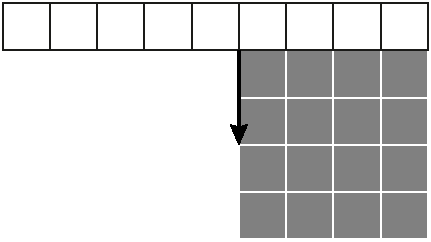
\includegraphics[width=9cm/2]{okt4-5.pdf}}
  \vspace*{1em}

  \subcaptionbox{\label{okt-d}}{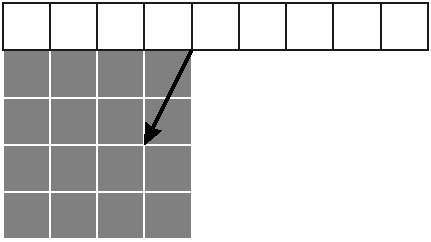
\includegraphics[width=9cm/2]{okt5.pdf}}
  \hfill
  \subcaptionbox{\label{okt-e}}{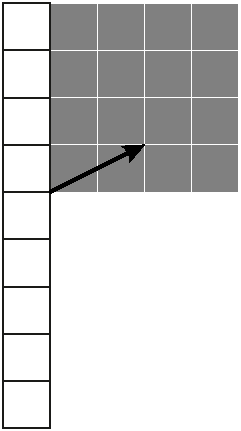
\includegraphics[width=5cm/2]{okt2.pdf}}
  \hfill
  \subcaptionbox{\label{okt-f}}{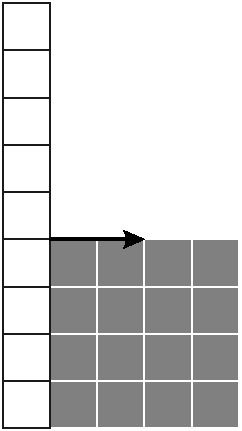
\includegraphics[width=5cm/2]{okt2-3.pdf}}
  \hfill
  \subcaptionbox{\label{okt-g}}{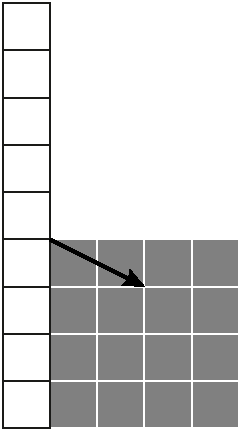
\includegraphics[width=5cm/2]{okt3.pdf}}
  \hfill
  \subcaptionbox{\label{okt-h}}{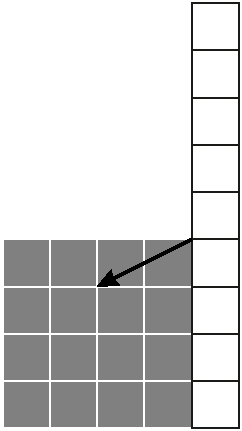
\includegraphics[width=5cm/2]{okt6.pdf}}
  \vspace*{1em}
  \caption{Poloha a~orientace pri\-már\-ního souseda v~zá\-vislosti na oktantu směr\-ového vektoru.}
  \label{fig:okt}
\end{figure*}

\begin{figure}[htbp]\centering
  \centering
  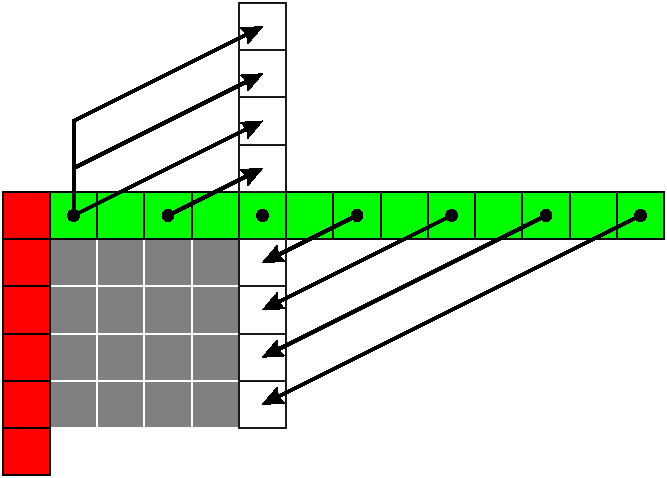
\includegraphics[width=14cm/2]{krok1.pdf}%
  \caption{Prvním krokem pre\-diktoru je promítnutí předpokládaných dostupných vzorků z~okolí na pri\-már\-ního souseda.}
  \label{fig:krok1}
\end{figure}

\begin{figure}[htbp]\centering
  \centering
  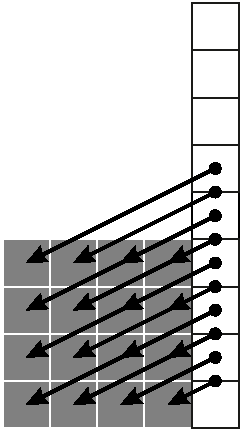
\includegraphics[width=5cm/2]{krok2.pdf}%
  \caption{Druhým krokem pre\-diktoru je promítnutí vzorků z~pri\-már\-ního souseda do bloku. Provádí se interpolace.}
  \label{fig:krok2}
\end{figure}


Intra pre\-dikce byla poprvé specifikována v~doporučení ITU-T H.261, a~to pro kom\-pre\-si 2D snímků videa.
Od té doby je v~různých formách nedílnou součástí drtivé většiny používaných kodeků pro vi\-deo\-kom\-pre\-si.
Novější specifikace se od starších liší zejména množstvím režimů intra kom\-pre\-se.
Největší pokrok lze pozorovat mezi specifikacemi ITU-T H.264 a~ITU-T H.265.
Doporučení ITU-T H.264 používalo devět pevně určených modů pre\-dikce, které byly specifikovány pro určité velikosti bloků.
Oproti tomu je v~ITU-T H.265 zavedeno 35 módů pre\-dikce, které se musí vypořádat s~dělením bloků do oktalových stromů (CTU).
H.265 zároveň zavádí vyhlazení referenčních vzorků pomocí FIR filtru, což má za následek zlepšení pre\-dikce a~lepší kom\-pre\-se.
Existuje mnoho publikací zabývajících se me\-to\-dou rychlé a~efektivní volby vhodného režimu intra pre\-dikce pro real-time kom\-pre\-si videa, ale žádná nezavádí pre\-dikci pro více-než-dvoudimenzionální bloky.
Tato práce proto pri\-már\-ně vychází z~poznatků již zmíněných doporučení ITU-T.

V~této práci je představeno řešení pro intra pre\-dikci libovolně dimenzionálních bloků, které je výsledkem zobecnění me\-to\-dy používané v~doporučení ITU-T H.265.
Řešení je rozděleno na dva kroky, přičemž každý krok řeší různé problémy, které vycházejí z~multidimenzionality dat.
V~prvním kroku jsou referenční vzorky $n$-dimenzionálního okolí promítnuty do $n-1$-dimenzionální roviny podle $n$-dimenzionálního směr\-ového vektoru.
V~tomto kroku je řešen problém nedostupného okolí, který se týká pre\-dikce okrajových bloků.
Navržené řešení poskytuje rozhraní pro volbu strategie výběru náhradních vzorků. Lze tak například použít nejbližší dostupný vzorek, případně nějakou pokročilejší formu interpolace.
V~$n-1$-dimenzionální rovině poté probíhá vyhlazení vzorků pomocí FIR filtru, podobně jako v~ITU-T H.265.
V~druhém kroku se vzorky z~pre\-dikovaného $n$-dimenzionálního bloku promítnou z~připravené $n-1$-dimenzionální roviny.
V~tomto kroku jsou již všechny vzorky vždy dostupné, takže tento krok je velmi rychlý.
Tento dvoukrokový přístup neredukuje časovou ani paměťovou náročnost algoritmu, ale velmi výrazně zjednodušuje implementaci algoritmu a~řešení okrajových případů.

Vstupem algoritmu je velikost pre\-dikovaného bloku, jeho dostupné okolí a~směr\-ový vektor, podle kterého se okolí rozšíří do bloku.
Platí, že každý $n$-dimenzionální blok má $2n$ $n-1$-dimenzionálních sousedů.
Algoritmus beze ztráty obecnosti předpokládá, že existuje $n$ sousedů, ze kterých je možné pre\-dikovat, a~jsou to vzorky s~příslušející souřadnicí nižší než souřadnice vzorků v~pre\-dikovaném bloku.
Pro dva roz\-měry je předpokládané okolí zaznačeno na obrázku~\ref{dost-a}.
V~případě potřeby lze algoritmus vždy zavolat s~invertovaným přístupem k~okolí a~invertovaným směr\-ovým vektorem tak, aby platil zmíněný předpoklad.
Z~tohoto předpokladu plyne, že alespoň jedna komponenta směr\-ového vektoru musí být kladná.

K~okolí příslušejícímu ne-kladné komponentě směr\-ového vektoru algoritmus vůbec nepřistupuje, pro korektní pre\-dikci nemusí vůbec existovat.
Obrázek~\ref{fig:kv} ukazuje, ke kterým vzorkům pre\-diktor přistupuje v~zá\-vislosti na kvadrantu směr\-ového vektoru.
Uživatel se na tento přístup může spolehnout, může například volat pre\-dikci jen pro takové vektory, pro které má dostupné okolí.
Alternativní možností uživatele je volat algoritmus nezá\-visle na dostupnosti vzorků a~poté pouze provádět korekce přístupu k~nim, pokud se o~to algoritmus pokusí.

Reálně se nedá předpokládat, že všechny vzorky z~předpokládaného okolí budou dostupné na straně dekodéru.
Pro průchod po řádcích je okolí dostupné na straně dekodéru zaznačeho na obrázku~\ref{dost-b}.
Obrázek~\ref{fig:dost-3D} zobrazuje vzorky dostupné na straně dekodéru pro kom\-pre\-si ve 3D.
Už ve třech roz\-měrech není na první po\-hled zřejmé, které vzorky jsou při průchodu po řádcích dostupné na straně dekodéru.
Pro průchod po řádcích v~libovolném počtu dimenzí platí, že kodér může v~daném roz\-měru přistupovat k~vzorkům z~následujících bloků pouze pokud v~jednom z~vyšších roz\-měrů zároveň přistupuje k~předcházejícím blokům.
Toto si lze snadno představit ve dvou roz\-měrech s~pomocí obrázku~\ref{dost-b}.
Prediktor může přistoupit k~vzorkům přesahujícím velikost bloku na horizontální ose pouze pokud na vertikální ose přistupuje \textit{do minulosti}.
Prediktor nemůže přistoupit k~vzorkům přesahujícím velikost bloku na vertikální ose, protože vertikální roz\-měr je nejvyšší.

Algoritmus se také musí vypořádat s~okrajovými případy, ve kterých nejsou potřebné vzorky dostupné ani na straně kodéru.
Takové případy přísluší krajním blokům komprimovaného obrázku, jak je demonstrováno na obrázku~\ref{fig:okraj}.
Při kom\-pre\-si světelných polí se ukázalo, že takto okrajovým případem je alespoň v~jedné dimenzi každý blok.
Tyto případy je proto nutné řešit více důkladně než při kom\-pre\-si ve 2D.
Tyto případy jsou opět řešeny na straně uživatele, který může volit vlastní strategii.
Podobně jako při problému dostupnosti při průchodu po řádcích může uživatel algoritmus volat jen s~takovými vektory, které nebudou přistupovat k~nedostupným vzorkům podle obrázku~\ref{fig:kv}.
Alternativní možností uživatele je volat algoritmus nezá\-visle na dostupnosti vzorků a~poté pouze provádět korekce přístupu k~nim.
Za korekci se v~tomto případě považuje přesměr\-ování na nejbližší dostupný vzorek.

Algoritmus začíná s~volbou pri\-már\-ní dimenze.
Za tu je prohlášena dimenze s~největší absolutní hodnotou prvku ve směr\-ovém vektoru.
Primární dimenze určuje tvar pri\-már\-ního souseda.
Primární soused je $n-1$-dimenzionální blok, do kterého je promítnuto veškeré předpokládané okolí.
Volba s~největší absolutní hodnotou zajistí, že všech $n$ $n-1$-dimenzionálních sousedů lze podle zvoleného směr\-ového vektoru promítnout do jednoho nejmenšího možného pri\-már\-ního souseda.
Například pro blok velikosti $4 \times 4 \times 8 \times 8)$ a~směr\-ový vektor $(1, -3, 2, -2)$ bude mít pri\-már\-ní soused velikost $8 \times 12 \times 12$.

Poloha a~orientace pri\-már\-ního souseda ve dvou roz\-měrech je pro všechny oktanty směr\-ového vektoru demonstrována na obrázku~\ref{fig:okt}.
Ze všech případů polohy pri\-már\-ních sousedů jsou nejvíce zvláštní případy~\ref{okt-a} a~\ref{okt-h}.
V~těchto případech pri\-már\-ní soused neleží v~rovině žádného existujícího souseda.
Pro správné pochopení kroků algoritmu budou tyto kroky vizualizovány právě na tomto případě.

Samotné promítnutí se provede rychle se zaokrouhlením na nejbližší celý vzorek.
Již v~ITU-T H.265 bylo zjištěno, že preciznější promítání přináší nemalé výpočetní nároky a~nemá vel\-ký vliv na kom\-pre\-si.
Tento krok je pro směr\-ový vektor z~obrázku~\ref{okt-h} demonstrován obrázkem~\ref{fig:krok1}.
Zelené vzorky představují předpokládané okolí, bílou barvou jsou zaznamenány vzorky primárního souseda.
Červenou barvou jsou zaznamenány vzorky, ke kterým pre\-diktor nemusí a~nesmí přistupovat, jelikož vektor spadá do případu~\ref{kv-e}.

Podobně jako v~ITU-T H.265 je pri\-már\-ní soused je před průmětem do bloku podroben $3^n$ Gaussově filtru.
Toto filtrování předejde případnému vzniku vysokých frekvencí v~reziduu a~má proto pozitivní vliv na kom\-pre\-si.
Toto chování bylo experimentálně potvrzeno.

Pomocí takto zpracovaného pri\-már\-ního souseda poté probíhá samotné promítnutí do bloku.
Tento krok je demonstrován obrázkem~\ref{fig:krok2}.
Každému vzorku v~bloku je pomocí inverzního směr\-ového vektoru na\-le\-zena pozice na pri\-már\-ním sousedovi, ze kterého je poté lineárně interpolována pre\-dikovaná hodnota vzorku.
V~tomto kroku je již zajištěno, že všechny potřebné vzorky jsou dostupné.

Navržená me\-to\-da je implementována jako modul pro využití v~kom\-pre\-sních řetězcích, které data kódují po blocích v~libovolném počtu dimenzí.
Očekávané využití me\-to\-dy je pro kom\-pre\-si 4D světelných polí, avšak řešení je dostatečně obecné na to, aby dokázalo pracovat se 3D volumetrickými (lékařskými) daty či s~běžnými 2D fotografiemi.
Navržené řešení je určeno pro kom\-bi\-na\-ci s~algoritmem, který dokáže volit módy pre\-dikce tak, aby bylo dosaženo požadovaného poměru rychlosti a~zkreslení.

\begin{figure}[htbp]\centering
  \centering
  \subcaptionbox{Světelné pole HaToy.\label{pred-a}}{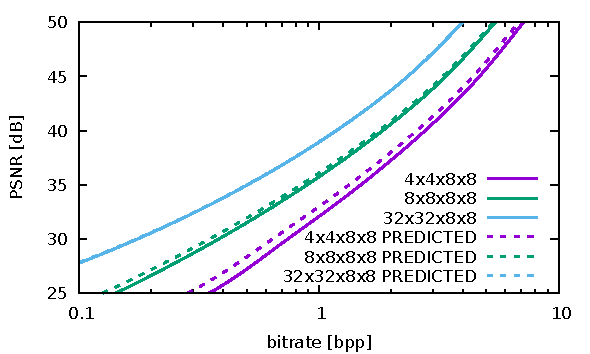
\includegraphics[width=\linewidth]{pred_HaToy.pdf}}\\
  \vspace*{1em}
  \subcaptionbox{Světelné pole Take2\_1. \label{pred-b}}{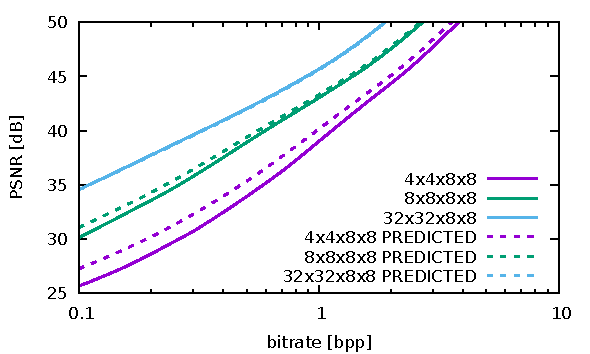
\includegraphics[width=\linewidth]{pred_Take2_1.pdf}}
  \vspace*{1em}
  \caption{Grafy demonstrují klesající efektivitu pre\-dikce s~rostoucí velikostí bloku.}
  \label{fig:pred}
\end{figure}

Modul byl integrován do existujícího kodéru světelných polí, který pracuje se čtyřroz\-měrnými hyperbloky obecných roz\-měrů (kapitola~\ref{hyperbloky}).
Pro každý blok je systematicky testováno 529 různých směrů, přičemž je zvolena pre\-dikce s~nejmenší absolutní chybou oproti originálnímu bloku.
Ke směr\-ové pre\-dikci je přidána také DC pre\-dikce a~planární pre\-dikce, která vzniká jako průměr dílčích směr\-ových pre\-dikcí s~bázovým vektorem.
Grafy~\ref{fig:pred} demonstrují, že takto integrovaná pre\-dikce redukuje bitrate jen pro menší bloky.
Testování hrubou silou zároveň navyšuje časovou náročnost o~ně\-ko\-lik řádů.
Autor proto navrhuje použít pre\-dikci v~kom\-bi\-na\-ci s~CTU.
Zároveň by se dalo diskutovat o~použití chytrého algoritmu, který by dokázal volit směr\-ové vektory na základě heuristiky.

\section{Hyperbloky obecných roz\-měrů} \label{hyperbloky}

Jedním z~největších omezení, kterými disponovalo přímé rozšíření kodéru JPEG do čtyř roz\-měrů, bylo použití hyperbloků pouze ve tvaru hyperkrychle.
Při správné velikosti bloku sice kódování dosahovalo dobré kom\-pre\-se, ale bylo zřejmé, že komprimovaná data mají v~úhlových dimenzích jinou povahu než v~pro\-s\-torových dimenzích.
Jedním z~logických kroků proto bylo existující kodér přepsat tak, aby dokázal využít hyperbloky libovolných roz\-měrů, které by poté bylo možné přizpůsobit komprimovaným datům.

Tato kapitola se zabývá popisem toho, co všechno změny zahrnovaly.
Nejdříve je popsáno, jak s~bloky funguje původní framework, jeho myšlenka, výhody a~nevýhody.
Jsou zhodnoceny návrhy, jak bylo možné problém řešit.
Dále je vysvětelno jakými změnami kodér prošel a~jaká úskalí to přineslo.
Je zhodnocen vliv jak na kom\-pre\-si, tak i~na časovou náročnost.
Kapitola končí výčtem možností, jak na tuto práci navázat a~co by mohlo řešit některé existující problémy.

Kodér byl v~základní variantě navržen s~myšlenkou statických bloků o~velikosti $8^4$.
To vycházelo z~kodéru JPEG, který používal bloky $8^2$.
Nebylo předokládáno, že by kodér mohl používat bloky jiných roz\-měrů, proto byl blok reprezentován datovou strukturou, která poskytovala čtyřroz\-měrné rozhraní k~jednoroz\-měrnému statickému poli o~velikosti 4096 prvků.
Tento přístup měl tu výhodu, že již při kompilaci šly do jisté míry zjistit paměťové nároky, kompilátor tak měl možnost v~případě potřeby provádět optimalizace.
Zároveň se tak dalo vyhnout dynamickým alokacím, které by v~prvních fázích vývoje mohly vést na větší chybovost.

Později se ukázalo, že bloky $8^4$ jsou nedostatečné, bylo proto rozhodnuto velikost bloku definovat pomocí šab\-lonového pa\-ra\-me\-tru v~jazyce C++.
Tímto způsobem bylo možné stále využívat statické pole pro data, ale velikost bloku bylo možné volit při kompilaci.
To vedlo k~tomu, že bylo potřeba přepsat do šab\-lon také veškerý kód, který takové bloky používá, zejména DCT a~cik-cak průchod.
Šablonový kód vedl na časově náročenější kompilaci, ale na druhou stranu umožňoval inlinovat funkce, u~kterých to dává smysl.

Ortogonálně k~tomu byl na základě častého experimentování s~jiným počtem dimenzí přidán šab\-lonový pa\-ra\-me\-tr pro počet dimenzí.
S~tím bylo spojené přepsání celého frameworku tak, aby byl schopný pracovat univerzálně, tedy s~libovolně dimenzionálními bloky libovolných roz\-měrů.
Byla to netriviální a~časově náročná úloha, která však vedla na minimalistický, dobře pochopitelný a~často rekurzivní kód, který bylo možné instancovat pro všechny potřebné experimenty s~blokovou kom\-pre\-sí.
Zároveň tím extrémně odlehčila způsobu přemýšlení ve čtyřech roz\-měrech, které vedlo na snažší řešení nových problémů.
Autorovi stačilo nový problém vyřešit ve dvou a~třech roz\-měrech, abstrahovat rekurzivní pattern a~otestovat, jestli platí i~pro 4D.

Taková implementace je sice silně univerzální, ale disponuje řadou nevýhod.
Tvar bloku je daný statickým pa\-ra\-me\-trem, uživatel si tak musí při kompilaci zvolit, jaké bloky bude používat.
Další nevýhodou je, že v~každé instanci se předpokládá kom\-pre\-se pomocí hyperkrychlí, což často nerespektuje povahu dat.
Tyto nevýhody například vylučují použití CTU, které ze své podstaty pracuje s~bloky různých velikostí.

První idea řešení byla z~jednoho šab\-lonového pa\-ra\-me\-tru udělat pole pa\-ra\-me\-trů, které určují velikost bloku.
Tento přístup by zachoval výhody statického bloku, ale zároveň i~jeho nevýhody, jeho roz\-měry by musely být známé při kompilaci.
Druhou možností bylo zavedení dynamické alokace.
Takové řešení by umožňovalo vytvoření libovolných bloků na požádání a~řádné zapouzdření by řešilo korektní správu paměti.
Toto řešení však vyvolávalo nedůvěru.
Nedalo se spoléhat, že dynamická alokace bude stejně rychlá jako zásobníková alokace.
Vzhledem k~častému vytváření nových bloků a~rušení starých, oproti znovupoužití, by to mohlo vést na nepříjemné zpomalení běhu, což by brzdilo už tak časově náročný proces validace kódu po každé změně.

Po zhodnocení byla zvolena dynamická alokace.
Dynamicky alokované pole bylo zapouzdřeno do šab\-lonové struktury, kde šab\-lonové pa\-ra\-me\-try specifikují datový typ vzorku a~počet dimenzí.
Velikost bloku je zadávána v~konstruktoru.
Změna zahrnovala refaktorizaci drtivé většiny kódu, která pracuje s~bloky.
Z~funkcí byl odstraněn šab\-lonový pa\-ra\-me\-tr pro velikost bloku, roz\-měry bloku jsou poskytovány v~jeho rozhraní nebo v~poli jako běžný pa\-ra\-me\-tr.
Přepsány byly jednotlivé kroky kom\-pre\-se.
Vzhledem k~jejich existující rekurzivní implementaci to většinou nepředstavovalo problém.

Vliv velikosti bloku na datový tok lze vyčíst z~ob\-ráz\-ku~\ref{fig:shift}.
Dynamická alokace se projevila jen $<~10\%$ ná\-růstem doby kom\-pre\-se a~dekom\-pre\-se.
Za tuto cenu bylo při správné volbě velikosti bloku u~některých obrázků dosaženo až $30\%$ redukce bitrate při stejné hodnotě PSNR.
Této redukce však bylo dosaženo pouze při prohledávání velikostí bloku hrubou silou.
Aktuálně proto problém spočívá v~tom, jak rychle a~efektivně najít optimální velikost bloku.
Zároveň se předpokládá, že se vyplatí navázat implementací CTU, která bude velikosti bloku volit podle lokálních změn v~obrázku.

Pro vyvážení zvýšených nároků dynamické alokace autor navrhuje implementaci zásobníkového alokátoru.
Taková implementace by však musela zajistit, že k~dealokaci bloků bude vždy docházet v~opačném pořadí oproti alokaci.
Alternativním řešením by mohl být předem alokovaný pool bloků různých typů.
V~obou případech by šlo využít faktu, že při spuštění programu jsou známé všechny informace o~počtu a~typu blokových bufferů, které bude kodér i~dekodér potřebovat.

\section{Vzájemný posun po\-hledů}\label{disp}

\begin{figure}[htbp]\centering
  \centering
  \subcaptionbox{Před vzájemným posunutím.\label{avg_Take2_1-a}}{
\includegraphics[width=.5\linewidth]{avg_Take2_1_original.png}}%
  \subcaptionbox{Po vzájemném posunutí.\label{avg_Take2_1-b}}{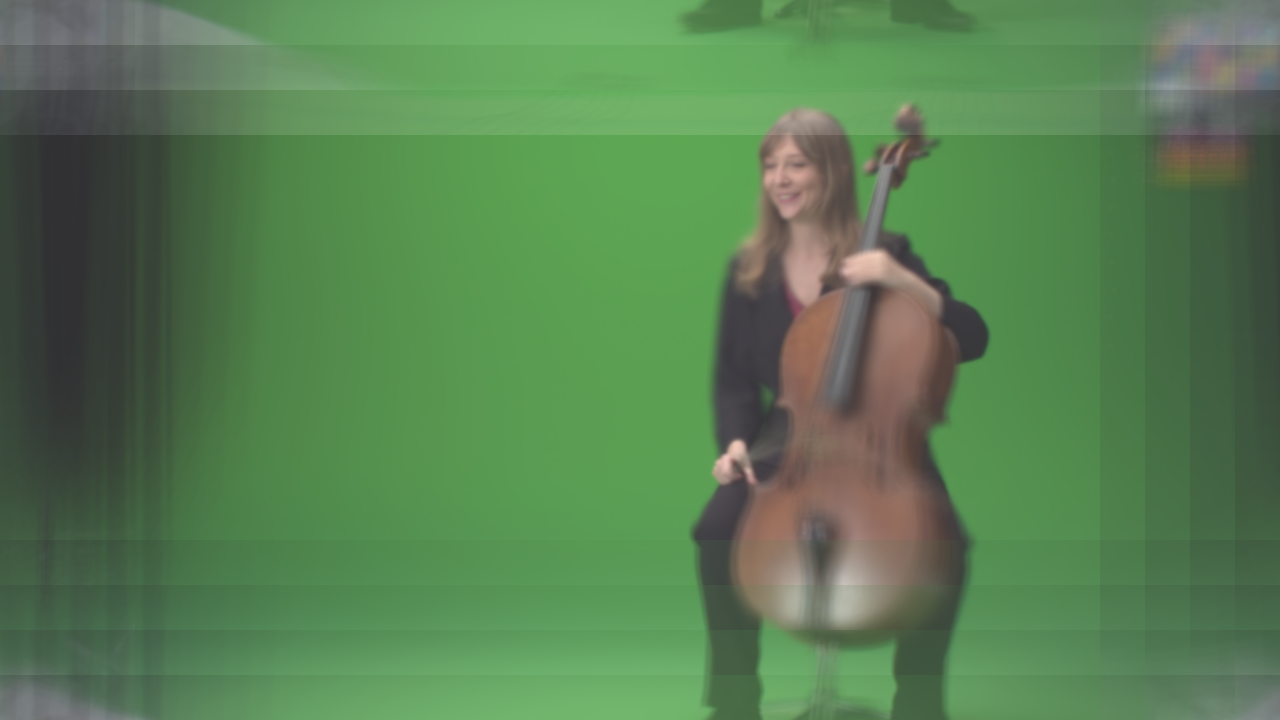
\includegraphics[width=.5\linewidth]{avg_Take2_1_shifted.png}}
  \vspace*{1em}
  \caption{Průměr ze všech po\-hledů ve světelném poli Take2\_1 před (\ref{avg_Take2_1-a}) a~po (\ref{avg_Take2_1-b}) vzájemném posunutí.}
  \label{fig:avg_Take2_1}
\end{figure}

\begin{figure}[htbp]\centering
  \centering
  \subcaptionbox{Před vzájemným posunutím.\label{avg_HaToy-a}}{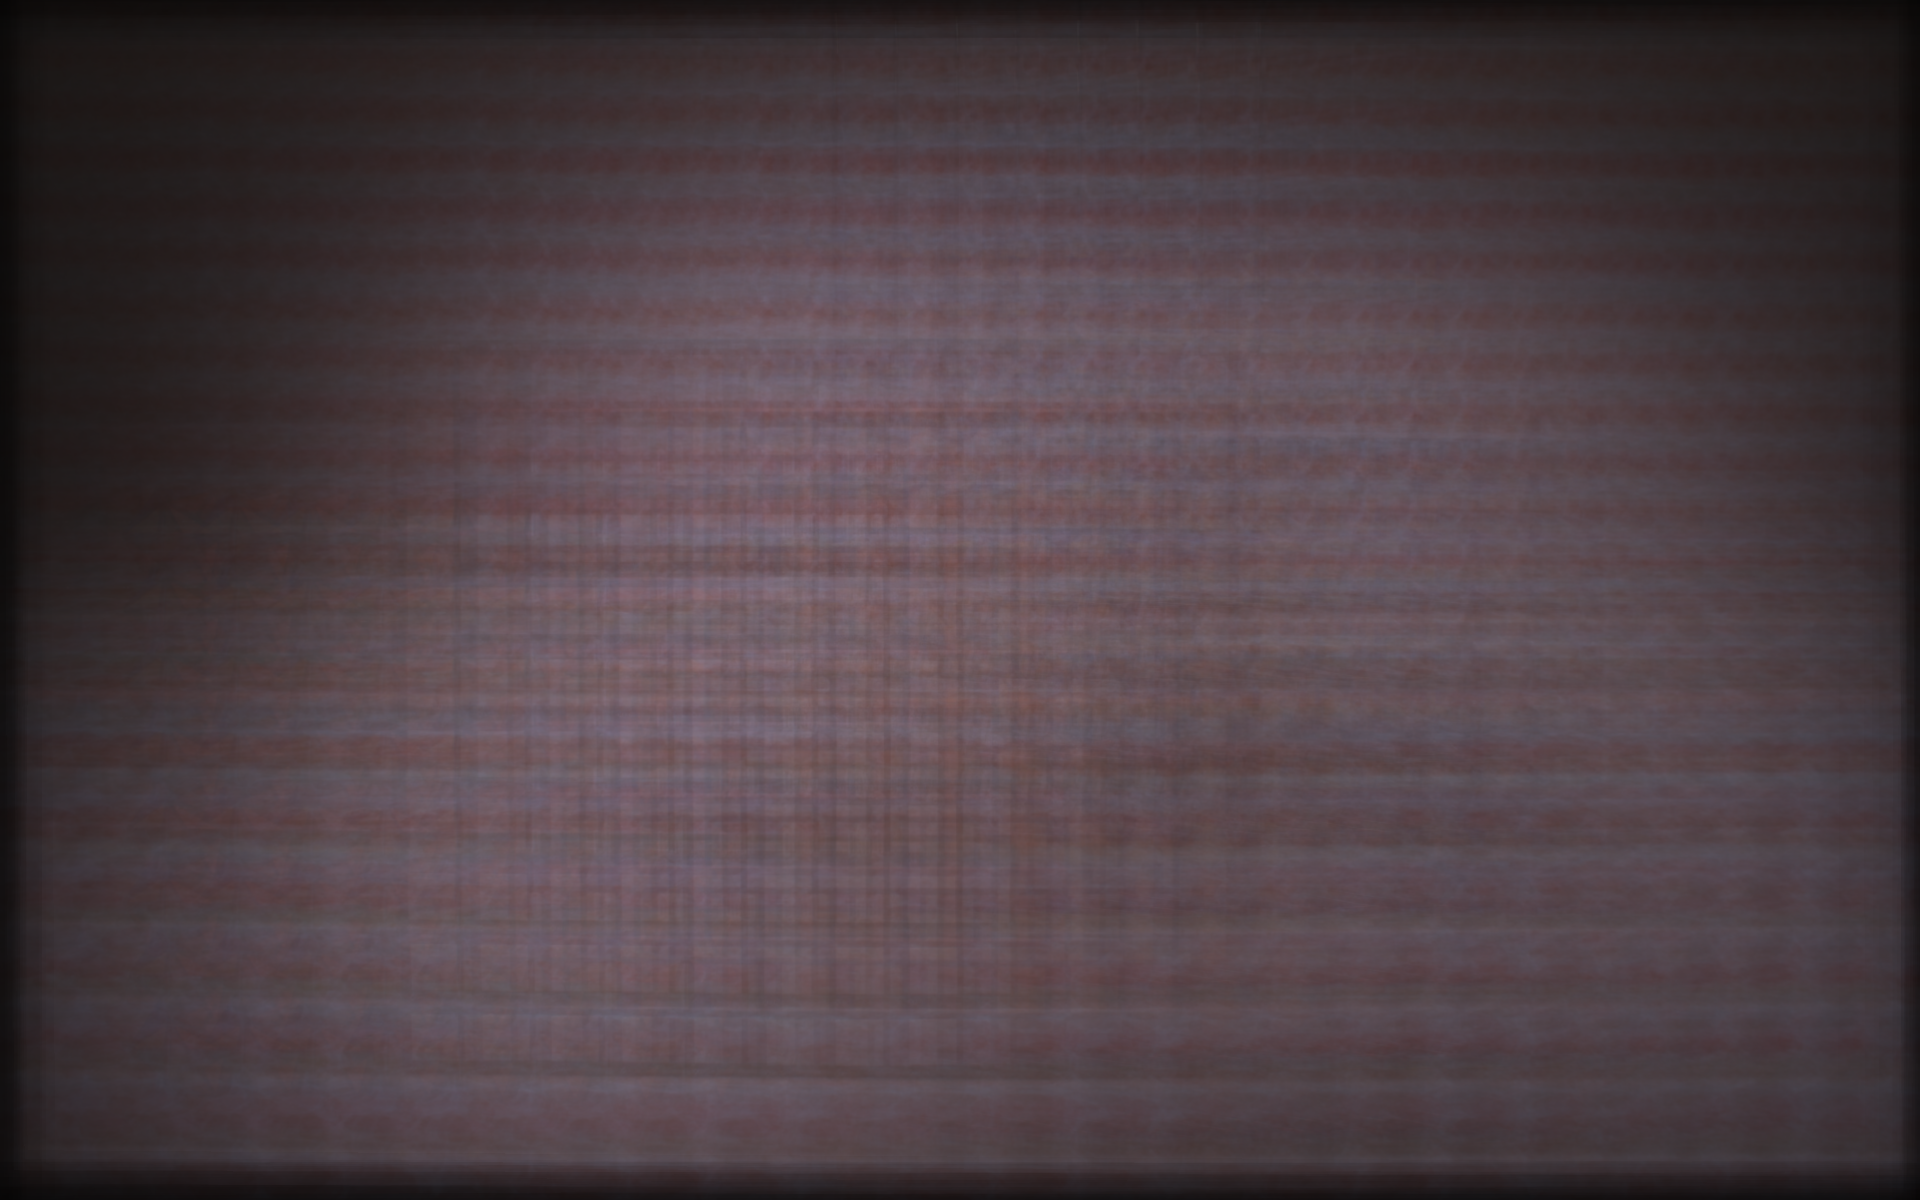
\includegraphics[width=.5\linewidth]{avg_HaToy_original.png}}%
  \subcaptionbox{Po vzájemném posunutí.\label{avg_HaToy-b}}{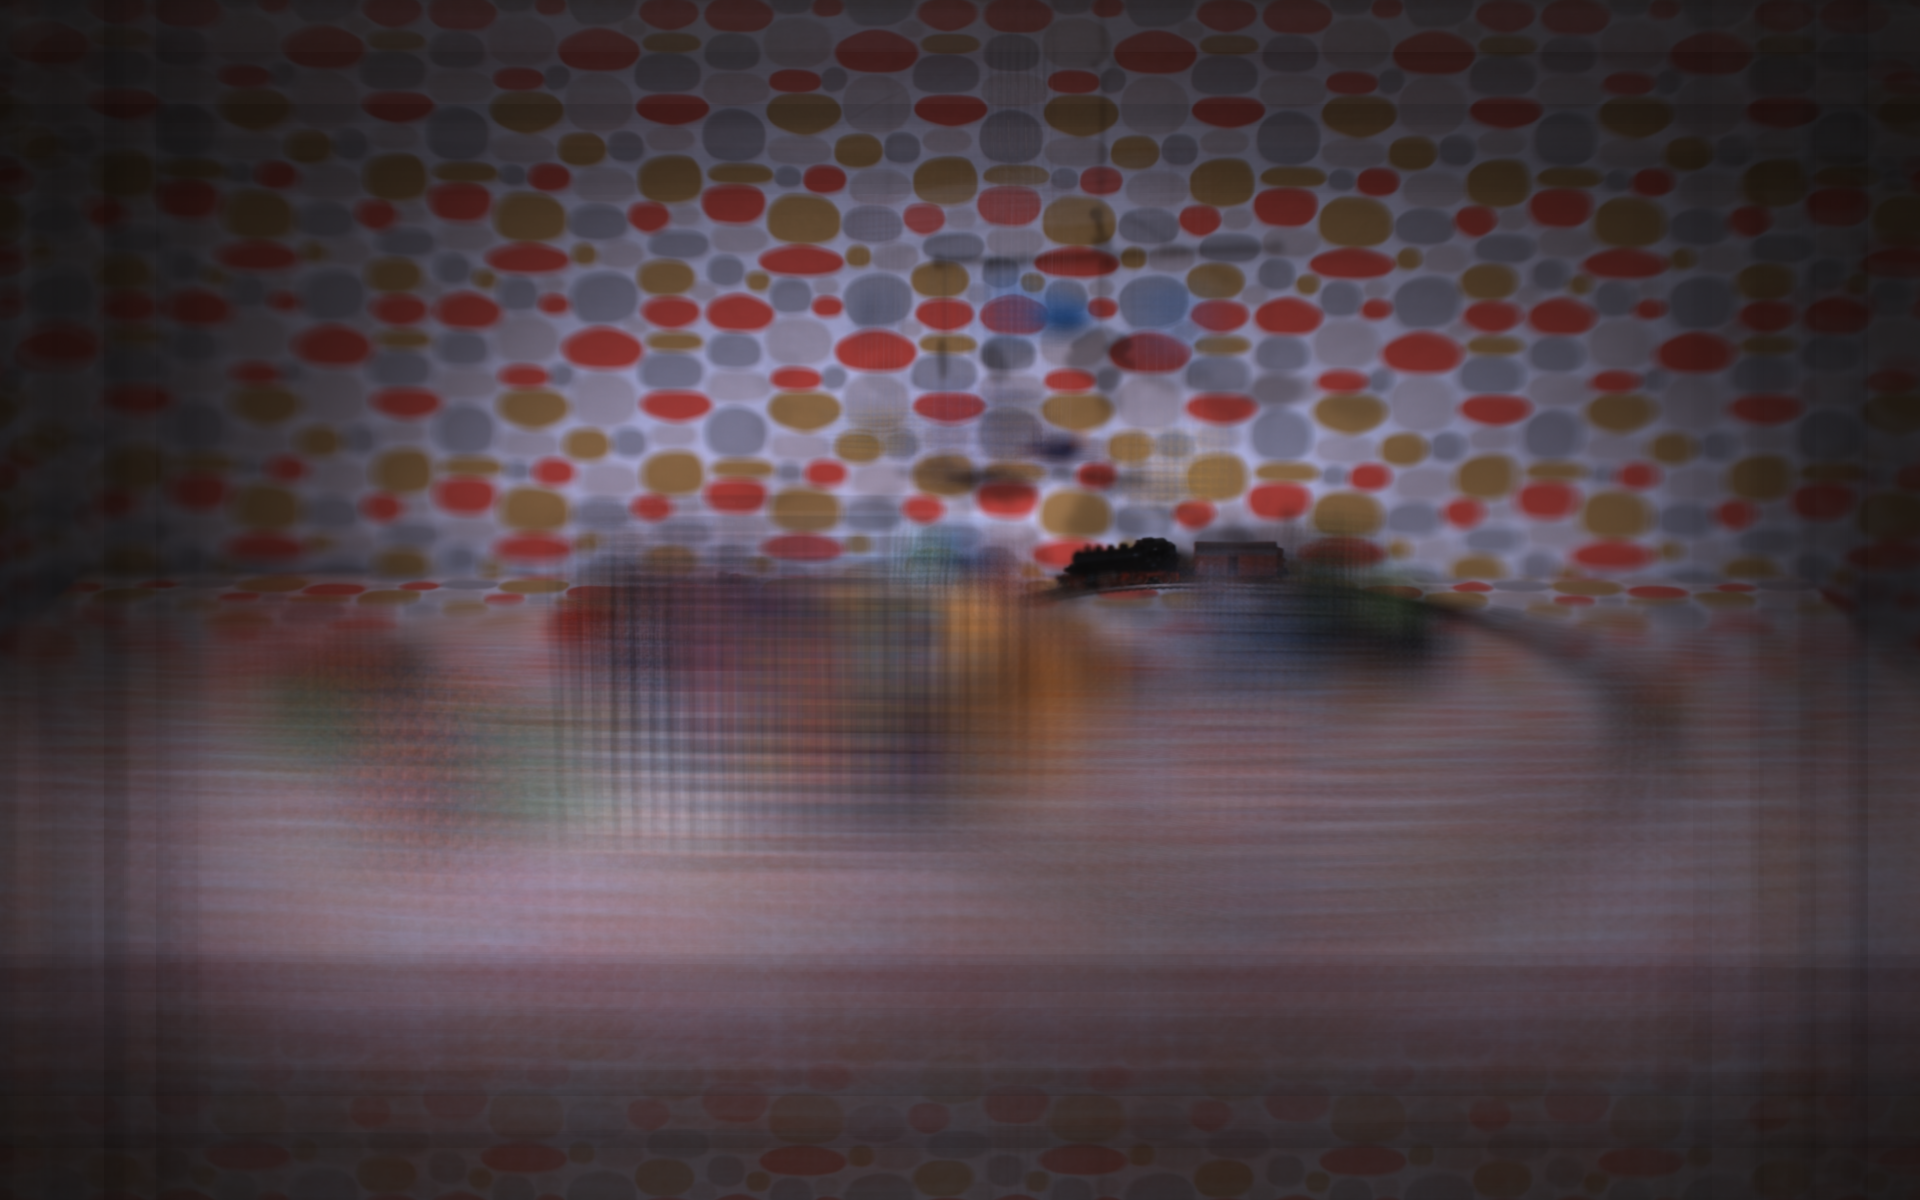
\includegraphics[width=.5\linewidth]{avg_HaToy_shifted.png}}
  \vspace*{1em}
  \caption{Průměr ze všech po\-hledů ve světelném poli HaToy před (\ref{avg_HaToy-a}) a~po (\ref{avg_HaToy-b}) vzájemném posunutí.}
  \label{fig:avg_HaToy}
\end{figure}

\begin{figure}[htbp]\centering
  \centering
  \subcaptionbox{Světelné pole HaToy.\label{shift-a}}{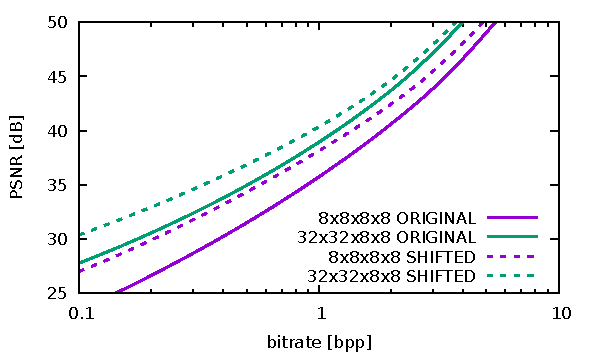
\includegraphics[width=\linewidth]{shift_HaToy.pdf}}\\
  \vspace*{1em}
  \subcaptionbox{Světelné pole Take2\_1. \label{shift-b}}{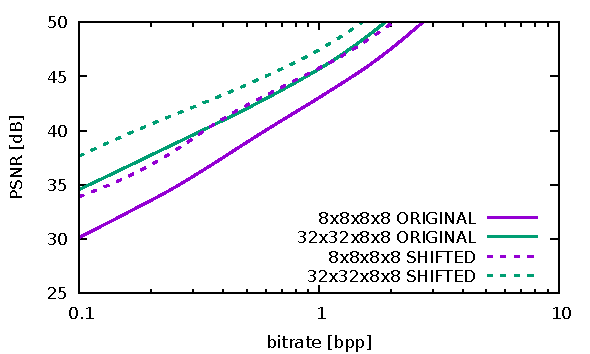
\includegraphics[width=\linewidth]{shift_Take2_1.pdf}}
  \vspace*{1em}
  \caption{Grafy demonstrující redukci datového toku po na\-le\-zení optimální velikosti bloku a~optimálního vzáhemného posunu.}
  \label{fig:shift}
\end{figure}

Čtyřroz\-měrné světelné pole reprezentuje paprsky světla procházející dvouroz\-měrným rozhraním ve troj\-roz\-měrném pro\-s\-toru.
Definice ovšem nic neříká o~tom, jaké má rozhraní tvar, velikost, jaký je rozsah a~hustota vzorkování v~pro\-s\-torové a~úhlové doméně.
Často se stává, že záznam světelného pole je rozostřený v~pro\-s\-torové doméně, což jde vidět na obrázku~\ref{avg_Take2_1-a} a~\ref{avg_HaToy-a}.
Jednotlivé po\-hledy tak sice můžou být vzájemně velmi podobné, ale o~ně\-ko\-lik pixelů posunuté.
To může vést až k~tomu, že hyperblok obsahuje z~každého po\-hledu jinou logickou část scény.
Vzorky tak v~rámci bloku nejsou korelované a~to vede na špatnou kom\-pre\-si.

Logickým krokem k~řešení tohoto problému je posunutí po\-hledů tak, aby se mezi nimi minimalizovala vzájemná chyba.
Jelikož se dá předpokládat, že po\-hledy byly zaznamenány pravidelným polem kamer, lze také předpokládat, že je posun stejný ve vertikálním i~horizontálním směru.
Zároveň lze předpokládat, že posun mezi libovolnými dvěma sousedními po\-hledy je vždy stejný.
Celý posun proto lze reprezentovat jednou hodnotou.

Středový po\-hled se prohlásí za fixní.
Každý po\-hled je v~horizontálním, resp. vertikálním směru posunut o~počet pixelů, který odpovídá hodnotě posunu vynásobené horizontální, resp. vertikální vzdáleností od středového po\-hledu.
Platí, že snímky horizontálně nalevo a~vertikálně nahoře mají zápornou vzdálenost.

Posunuté vzorky polohou přesahující roz\-měry po\-hledu jsou rolovány do pomyslného torusu pomocí operace modulo.
Tato operace ve výsledném obrázku tvoří vysoké frekvence kolem okrajů a~v~zá\-vislosti na velikosti posunu obsahují okraje po\-hledů vzájemně nekorelovaná data.
Z~po\-hledu blokového kodéru to však nevadí, pokud v~rámci jednoho bloku nejsou korelovaná ani původní data.
V~takovém případě dojde z~po\-hledu kodéru pouze ke zvýšení průměrné korelace a~tím i~zlepšení kom\-pre\-se.
Nevýhodou je, že po dekom\-pre\-si můžou mít okraje horší kvalitu než střed obrázku.
Vliv posunutí na ostrost v~pro\-s\-torové doméně lze pozorovat na obrázcích~\ref{fig:avg_Take2_1} a~\ref{fig:avg_HaToy}.
Oba tyto obrázky jsou v~základu pro\-s\-torově rozostřené.
U~obrázku~\ref{fig:avg_HaToy} lze navíc pozorovat, že pro účely kom\-pre\-se bylo v~tomto případě lepší zaostřit na rozsáhlou část scény (tapetu) oproti části podstatné.

Implementovaný posun v~aktuální verzi pracuje s~celými pixely.
Při návrhu bylo zvažováno, jestli má být umožněn posun o~necelý počet pixelů v~kom\-bi\-na\-ci s~interpolací.
Od tohoto návrhu bylo upuštěno.
Experimenty ukázaly, že posun na sub-pixelové úrovni má zanedbatelný vliv na kom\-pre\-si, interpolace je časově náročná a~navíc ztrátová.

Vliv posunutí na datový tok lze vypozorovat z~ob\-ráz\-ku~\ref{fig:shift}.
Z~vyhodnocení plyne, že pro obrázky, které jsou originálně rozostřené v~pro\-s\-torové doméně dokáže posun redukovat bitrate až o~$45 \%$ při stejné kvalitě.
Nejvíce se posun projevuje na obrázcích z~datasetu SAUCE, které jsou zachyceny polem kamer.
Oproti tomu pro obrázky z~fotoaparátu Lytro, které mají disparitu mezi snímky menší než jeden pixel, je optimální hodnota posunu nula, tím pádem je pro ně tento krok irelevantní.
Je zřejmé, že tato pre-processingová operace nedokáže spasit každý špatně komprimovatelný snímek.
Pouze upraví existující data do podoby, která je lépe komprimovatelná blokovou me\-to\-dou.

Posun neřeší volbu jeho hodnoty.
Tu je potřeba před kom\-pre\-sí zjistit, liší se pro každý obrázek.
Bylo proto navrženo použití golden-section search pro vyhledání minima absolutní chyby mezi sousedními po\-hledy.
Experimentálně bylo zjištěno, že absolutní chyba mezi sousedními snímky koreluje s~výsledným datovým tokem.
Platí tak, že menší chyba vede na menší datový tok.
Golden-section search nalezne pouze jedno lokální minimum.
Experimenty ukázaly, že pokud má obrázek více lokálních minim, tak je s~nimi dosaženo srovnatelných datových toků.
Vyhledávání je implementováno na rozsahu posunů od záporné do kladné maximální zvolené hodnoty velikosti bloku v~úhlové doméně, například $\langle -8; 8~\rangle$ pro bloky o~velikosti $4\times8\times16\times16$.
Experimenty také ukázaly, že měření chyby mezi po\-hledy me\-to\-dou Monte Carlo dokáže zásadně redukovat čas vyhledávání optimálního posunu bez zásadního vlivu na výsledek.

%--------------------------------------------------------
%--------------------------------------------------------
%--------------------------------------------------------
%--------------------------------------------------------
\section{Závěr}
\label{sec:Conclusions}
Tato práce se věnovala zkoumání různých me\-to\-d, pomocí kterých by bylo možné vylepšit kom\-pre\-si 4D světelných polí.

Byl navržen a~implementován robustní algoritmus pro směr\-ovou intra pre\-dikci pro libovolně dimenzionální bloky.
Tento algoritmus se dokáže vypořádat s~řadou okrajových případů.
Reálnou dostupnost dat algoritmus neřeší, ale dává možnost uživateli volit strategii doplnění dat nedostupných.
Tento algoritmus lze zavolat nad libovolným $n$-dimenzionálním směr\-ovým vektorem pro pre\-dikci $n$-dimenzionálního bloku.

Navržený pre\-dikční algoritmus neřeší volbu optimálního směr\-ového vektoru.
S~rostoucím počtem dimenzí exponenciálně roste i~počet možných vektorů.
Na tuto práci je proto možné navázat návrhem optimalizační me\-to\-dy, která bude směr\-ový vektor volit v~rozumném čase.
Experimenty ukázaly, že směrová pre\-dikce redukuje datový tok pro bloky menších roz\-měrů.

Byl modifikován existující kodek světelných polí, který nyní umí zpracovávat obrázek po hyperblocích obecných roz\-měrů.
Tato modifikace umožňuje jemnější volbu velikosti bloku a~tím pomáhá dosáhnout lepšího kom\-pre\-sního poměru.
Na tuto modifikaci je možné navázat implementací dělení bloků do stromové struktury (CTU).
Volba vhodných roz\-měrů bloků dokáže redukovat bitrate až o~$30 \%$.

Byl zkoumán vliv vzájemného posunu mezi po\-hledy na datový tok.
Ukázalo se, že u~některých obrázků lze po\-hledy zaostřit na nejvíce obsáhlý objekt ve scéně a~dosáhnout tak redukce datového toku.
Hledání optimální hodnoty posunu je prováděno pomocí golden-section vyhledávání tak, aby byla minimalizována absolutní chyba mezi po\-hledy.
Vzájemný posun pohledů v~obrázku dokáže pro jisté případy redukovat datový tok až o~$45 \%$.

Plánem pro navazující projektovou praxi je implementace dělení bloků do stromové struktury (CTU) a s tím související návrh nového entropického kodéru.
V kombinaci s intra predikcí to povede na lepší dynamické přizpůsobení kodéru na kódovaná data a tím i na zvýšení kompresního výkonu.

\section*{Poděkování}
Rád bych poděloval svému vedoucímu Ing. Davidu Bařinovi, Ph.D. za jeho trpělivost v~dobách, kdy produktivita práce na této projektové praxi klesala na nulu.
